\documentclass[conference]{IEEEtran}
\IEEEoverridecommandlockouts
\usepackage{cite}
\usepackage{amsmath,amssymb,amsfonts}
\usepackage{algorithmic}
\usepackage{graphicx}
\usepackage{textcomp}
\usepackage{xcolor}
\usepackage{multirow}
\def\BibTeX{{\rm B\kern-.05em{\sc i\kern-.025em b}\kern-.08em
    T\kern-.1667em\lower.7ex\hbox{E}\kern-.125emX}}
\begin{document}

\title{Smart Spreading Factor Assignment for LoRaWANs}


\author{\IEEEauthorblockN{Tugrul Yatagan\IEEEauthorrefmark{1} and Sema F. Oktug\IEEEauthorrefmark{2}}
\IEEEauthorblockA{Department of Computer Engineering,
Istanbul Technical University\\
Istanbul, Turkey\\
Email: \IEEEauthorrefmark{1}yatagan@itu.edu.tr, \IEEEauthorrefmark{2}oktug@itu.edu.tr}}
\maketitle


\begin{abstract}
Low power wide area network (LPWAN) technologies offer affordable connectivity to massive number of low-power devices distributed over very large geographical areas using license-free frequency bands. Focus of this work is one of the most promising LPWAN technologies: LoRa. LoRa offers long range communication and strong resilience to interference by proprietary modulation technique based on Chirp Spread Spectrum. LoRa trades data rate for sensitivity and communication range by spreading symbols within a fixed channel bandwidth. Collisions in LoRaWAN networks are strongly related with spreading factor (SF) assignment of nodes which indeed effects network performance. In this work, a simulation environment to study different SF assignment schemes is implemented. Furthermore, novel SF assignment strategy is proposed which utilizes a machine learning technique for optimization. Finally, promising simulation results for proposed machine learning SF assignment technique is presented.
\end{abstract}


\begin{IEEEkeywords}
LoRa, Spreading Factor, IoT, LPWAN, Machine Learning
\end{IEEEkeywords}


\section{Introduction}
\par In the last few years, number of Internet of Things (IoT) applications increased exponentially \cite{7721743}. Recent developments on LPWAN technologies has great impact on growth of number of IoT applications. LPWAN technologies addresses some of the well-known wireless communication challenges. Traditional wireless communication methods such as cellular networks (e.g., 2G, 3G, LTE) and short-range communication (e.g., Bluetooth, WiFi, Zigbee) cannot provide low power and long range at the same time. Cellular networks can provide long range and high data rate but they are complex and consume too much power. Besides, most of the IoT applications do not require high data rate. Short-range communication methods can provide relatively low power consumption but their range is limited to a few hundred meters at best \cite{7815384}. LPWAN technologies fill the technology gap between short range and cellular communication by providing low power and long range communication. LPWAN technologies basically sacrifice data rate to provide low power consumption.

\par There are several emerging LPWAN technologies. LoRa, Sigfox, NB-IoT and LTE-M are commonly used, well-known LPWAN technologies. LoRa and Sigfox use license free ISM frequency bands while NB-IoT and LTE-M use licensed frequency bands which brings extra cost \cite{7815384}. Both LoRa and Sigfox are known for ultra low power consumption and resilient to interference while NB-IoT and LTE-M are promoted for higher data rate. LoRa has open standard MAC protocol called LoRaWAN. LoRaWAN and Sigfox MAC protocols are based on pure ALOHA medium access. LoRaWAN networks can be deployed as a private network. However, Sigfox and NB-IoT are only available with operator contracted deployments \cite{7815384}. Number of messages that Sigfox end device can send in a day is limited to 140 packets for uplink and just 4 packets for downlink. Also, Sigfox packet payload is limited to 12 bytes for uplink and 8 bytes for downlink. However LoRa supports up to 243 bytes payload and NB-IoT supports up to 1600 bytes payload. Sigfox maximum data rate is 100 bps, on the other hand maximum data rate for LoRa and NB-IoT are 50 kbps and 200 kbps respectively \cite{7815384}.

\par LoRa can adjust data rate by spreading symbols within a fixed channel bandwidth. This enables tradeoff between receive sensitivity and transmission time on air \cite{7803607}. LoRa supports 6 different SF option. Simultaneous same SF transmissions are prone to collision however different SF transmissions in same channel are orthogonal to each other up to some extent, thus SF assignment is crucial for overall network performance. In this work, a custom made LoRa discrete event simulator is introduced to study different LoRa SF assignment strategies. We also proposed an SF assignment scheme to increase network performance with the help of machine learning methods and we verified our proposal using the simulator.

\par The following two sections provides an background information about LoRaWAN and LoRa. Section \ref{Other Related Works} describes other related works. Section \ref{Proposed Technique} describes proposed technique for SF assignment. Simulation environments and results are shown in Section \ref{Simulation Environment} and \ref{Simulation Results}. Finally, Section \ref{Conclusion} concludes the paper.


\section{LoRaWAN} \label{LoRaWAN}
\par LoRa is a wireless link technology for LPWAN applications. LoRa has an open standard MAC protocol called LoRaWAN. LoRa and LoRaWAN terms are frequently and incorrectly used for each other.

\par LoRaWAN is a medium access control (MAC) layer protocol which designed for large scale LoRa networks. LoRaWAN is an open source standard developed and maintained by LoRa Alliance. LoRa Alliance is an open, non-profit organization dedicated to standardization of LoRaWAN. LoRa can be used without LoRaWAN as a wireless link technology, however LoRaWAN is developed considering well known LPWAN challenges and their best practice solutions. LoRaWAN also provides inter-operability between different LoRa networks. LoRaWAN is based on pure ALOHA medium access. LoRaWAN provides lightweight but powerful standard for wide range of LoRa IoT applications.

\par A typical LoRaWAN network consist of three network entities.

\subsection{End node}
\par LoRaWAN end node (EN) is low power embedded device that communicates to gateways. LoRaWAN standard defines three classes for end devices which are Class A, Class B, and Class C for providing LPWAN solution to different scenarios. Class A end nodes generates uplink transmission at any time and only receives a period of time after uplink transmission. Class B end nodes extend Class A by adding scheduled receive windows for downlink transmission. Receive window is synchronized using beacon packet transmitted by gateway. Class C end nodes extend Class A by keeping receive window open unless they are transmitting. This provides low latency donwlink communication but requires more power consumption. In this paper, we focused on Class A end devices since Class A provides lowest power consumption.

\subsection{Gateway}
\par LoRaWAN gateway (GW) is device that receive/transmit packets coming from/to end nodes. A typical gateway can receive from multiple channel at the same time. Gateways are typically connected to power grid so power consumption of a gateway is insignificant most of the deployments.

\subsection{Network server}
\par LoRaWAN network server (NS) is server that provides MAC layer processing. Network server routes messages from application to end nodes, and vice versa. Network server can be used for tweaking end node parameters like channel, transmit power, SF to increase network performance.


\section{LoRa}
\par LoRa is the name of the proprietary physical layer radio and chipset technology that provides wireless link solution for low power wide area networks. LoRa is designed and patented by Semtech Corporation. LoRa uses proprietary spread spectrum modulation technique that is derivative of Chirp Spread Spectrum (CSS). Chirp is a sinusoidal signal which its  frequency increases over time. The chirp frequency increases linearly and sweeps entire bandwidth. We invite readers to refer to \cite{AN1200.22} for further details.

\subsection{Spreading Factor}
\par Spreading factor (SF) is the ratio between symbol rate and chip rate. The ratio between symbol and chip rate is equal to $2$\textsuperscript{SF}. SF can take values between 7 to 12. SF also determines data rate of a LoRa transmission \cite{AN1200.22}.

\begin{equation} \label{eq:bit_rate_sf}
R_{b}|_{bps} = SF * \dfrac{\left[ \dfrac{4}{4+CR} \right] }{ \left[ \dfrac{2^{SF}}{BW|_{Hz}} \right]}
\end{equation}

Where, SF is spreading factor $SF \in \{7,..,12\}$, CR is error correction code rate $CR \in \{1,..,4\}$ and $BW$ is bandwidth in Hertz \cite{AN1200.22}.

\par While BW and CR are constant, as the SF increases the data rate decreases. Increasing SF makes the signal more resilient to noise thus increases the transmission range. Increasing SF also increases transmission duration which increases power consumption. Therefore it is possible to trade between data rate, range and power consumption by  changing SF.

\subsection{Spreading Factor Assignment Issue}
\par Simultaneous different SF transmissions are orthogonal to each other up to some extent. Which means, a LoRa gateway can simultaneously receive multiple transmissions with different SFs. However, simultaneous transmissions with same SF may not be received by gateway due to collision. For this reason, spreading factor assignment of nodes is crucial for network performance.

\par Initially, a node is not aware of how far it is from a GW. However, a node can guess how far away from the gateway by observing received signal power of a downlink transmission. If a downlink transmission received signal power is too high then node can decrease its next transmission SF or transmit power to decrease power consumption. Also GW can request from a node to decrease node's SF or transmit power. This SF assignment method is called lowest possible SF assignment scheme for the rest of the paper.

\par In Figure \ref{fig:collision}, a LoRaWAN network distributed around a single GW is illustrated. Different color rings represent achievable range of different SF from GW and different color circles represent nodes with selected SF. Most of the end devices which close to the GW will fall into lowest SF (SF7) area section. End devices which close to the GW will probably select lowest SF all the time. Which results a lot of collisions between same SF transmissions. Collision number increases while number of end devices close to the GW increases.

\begin{figure}
\centering
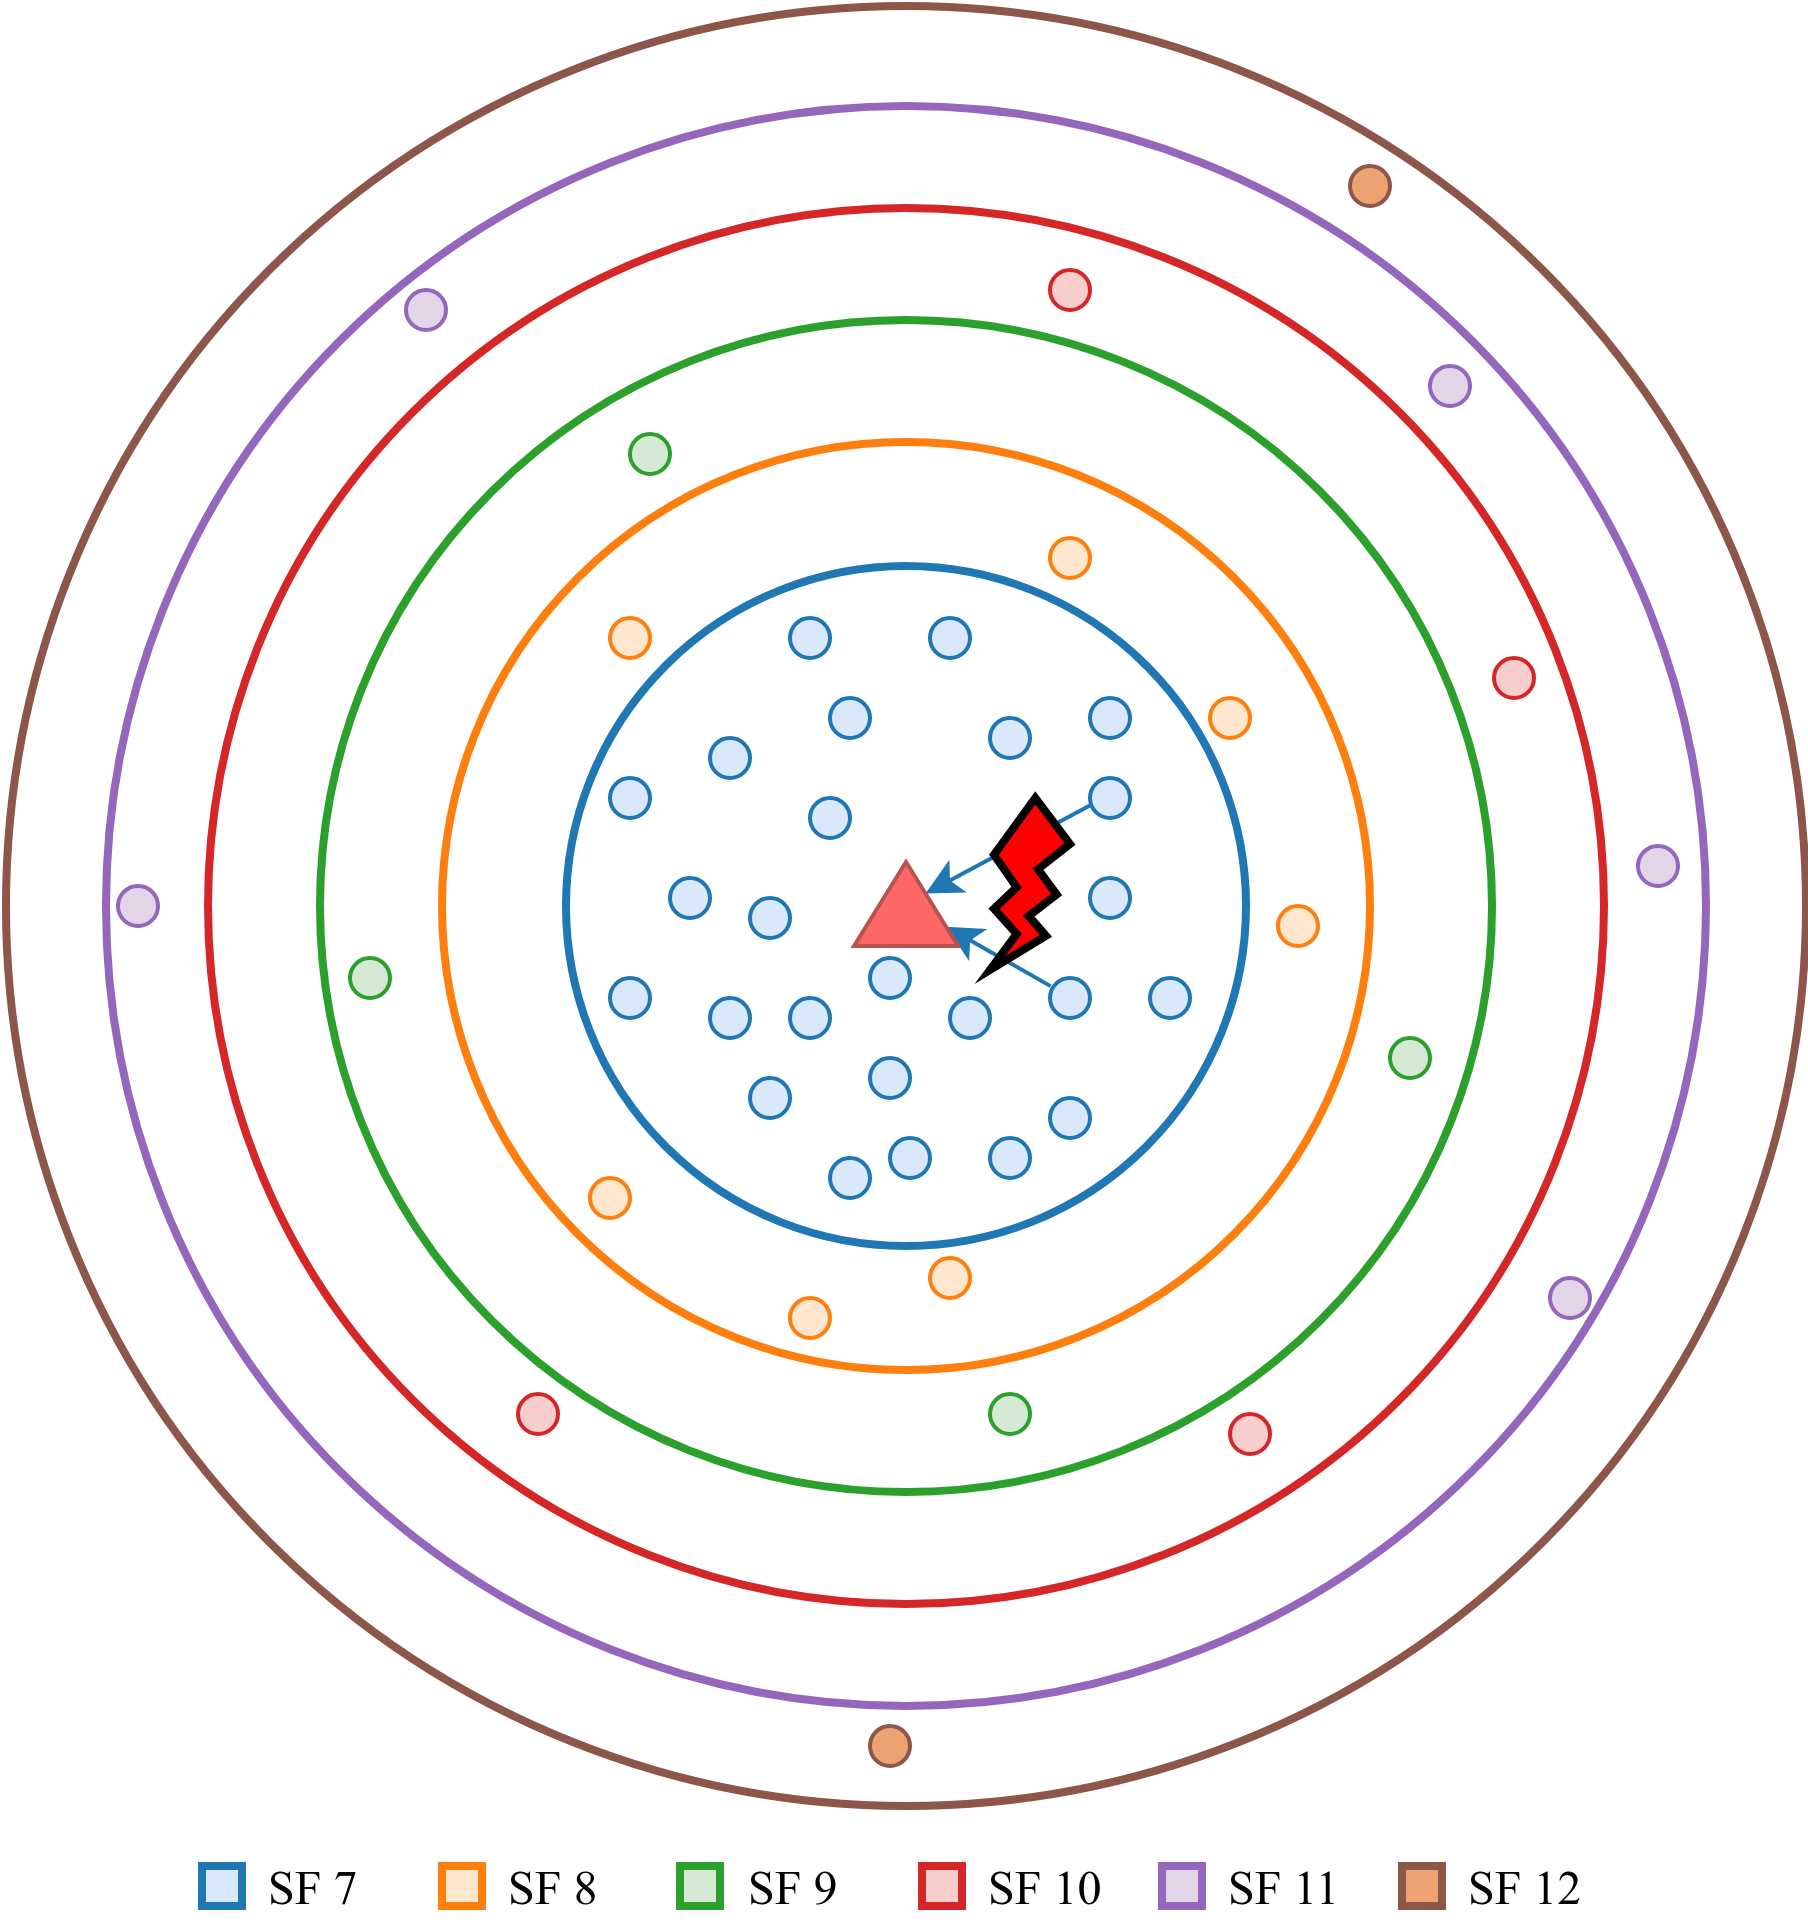
\includegraphics[width=\linewidth]{collision}
\caption{Collision between nodes close to the GW.}
\label{fig:collision}
\end{figure}


\section{Other Related Works} \label{Other Related Works}
The literature related to the work presented in this paper has started growing recently. LPWAN technologies and especially LoRa/LoRaWAN attract researchers attention lately. We listed some of these works which studying LoRaWAN and LoRa SF.

\par In \cite{7996384}, the authors evaluated the performance of LoRa networks in a smart city scenario. The
authors proposed a link measurement and a link performance model for LoRa. The authors also proposed a SINR threshold matrix for modeling LoRa interference between simultaneous but different SF LoRa transmissions. They implement a LoRa simulator in ns-3 to study scalability and performance of LoRaWAN networks. Their results show that LoRaWAN networks scale well as the number of nodes and gateways increases. They also show that SF assignment has great effect on network performance.

\par In \cite{8090518}, another LoRaWAN ns-3 simulator is presented. Authors introduced an error model for determining range as well as interference between multiple simultaneous LoRa transmissions. Their simulator supports LoRaWAN Class A end devices, multiple gateways, both upstream and downstream confirmed messages. Their results show that allocating network parameters to end devices is hugely important for the performance of LoRaWAN networks.

\par In \cite{s17061193}, the authors investigated single gateway LoRaWAN network scalability in terms of the number of end nodes using a simulation model based on real measurements. They measure the impact of two concurrent LoRa transmissions on each other by using physical LoRaWAN end devices and a gateway then they created a simulation model from measurements. Their results show that LoRaWAN has better scalability than pure ALOHA since a LoRa packet may still go through under collision if the the last six symbols of preamble and header of the packet does not collide.

\par In \cite{8267219}, the authors studied imperfect orthogonality between different LoRa SF transmissions. The authors state that a LoRa transmission can be interfered even between different SF transmissions when power of the interfering signal significantly overcomes the reference signal. Their experimental results show that this power difference is around 16 dB and this power difference can be seen when  interferer is close to receiver or multiple interferer can create this power difference cumulatively. 

\par In \cite{8430542}, the authors investigated the impact of interference caused by simultaneous LoRa transmissions using the same SF as well as different SFs. They derived aggregated co-SF and inter-SF interference power SIR distributions to capture the coverage performance with respect to the distance from the gateway for modeling interference in multiple gateway scenarios. Their results show that transmission among different SFs can cause a significant impact in high-density LoRaWAN networks.


\section{Proposed Technique} \label{Proposed Technique}
\par The collision issue illustrated in Figure \ref{fig:collision} can be solved if the GW force some of the close end nodes to select higher SF even if they can able to communicate with lower SF. This may result lower collisions due to the orthogonality of different SF as shown in Figure \ref{fig:collision_solution_single_gw}. Higher SF assigned nodes are drawn with bold circle border in Figure \ref{fig:collision_solution_single_gw}. However, how GW assign SF to which node becomes an another issue. Increasing a node's SF should be done carefully since higher SF means higher time on air and higher time on air is more prone to collision with other higher SF transmissions. In multiple GW scenarios, this approach may increase the collision number with nodes in other GW's range. Thus, extra care must be taken for nodes in intersection area of GWs illustrated in Figure \ref{fig:collision_solution_multi_gw}.

\par It is difficult to propose a single SF assignment rule for every possible LoRaWAN topology since every network is different and optimizing their nodes SFs requires different rules. For this reason, we proposed a machine learning based SF assignment scheme to decrease same SF transmission collision number.  This technique learns nodes behavior of a network. A NS can keep track of successful uplink transmission from nodes and their SFs. NS can also keep track of some of the collided transmission if header part of the packet does not interfered at GW. However, NS cannot keep track of transmissions with receive power lower than GW sensitivity. Using these obtained information NS can train a classifier for predicting transmission result for specific node and specific SF input. Using this predictor GWs can assign the lowest possible SF to nodes considering the collision probability.

\par In this work, we used decision tree classifier to predict transmission results. We utilized Gini index criteria to measure quality of decision tree splits and used balanced class weights. As most of the machine learning applications, increasing data set size increases prediction accuracy. For our case, data set size is directly proportional to simulation duration. Thus increasing simulation duration, increases the prediction accuracy. For real world cases, NS can keep track of transmission and it can create a classifier daily basis, then GW can request from nodes to use this new SF.

\begin{figure}
\centering
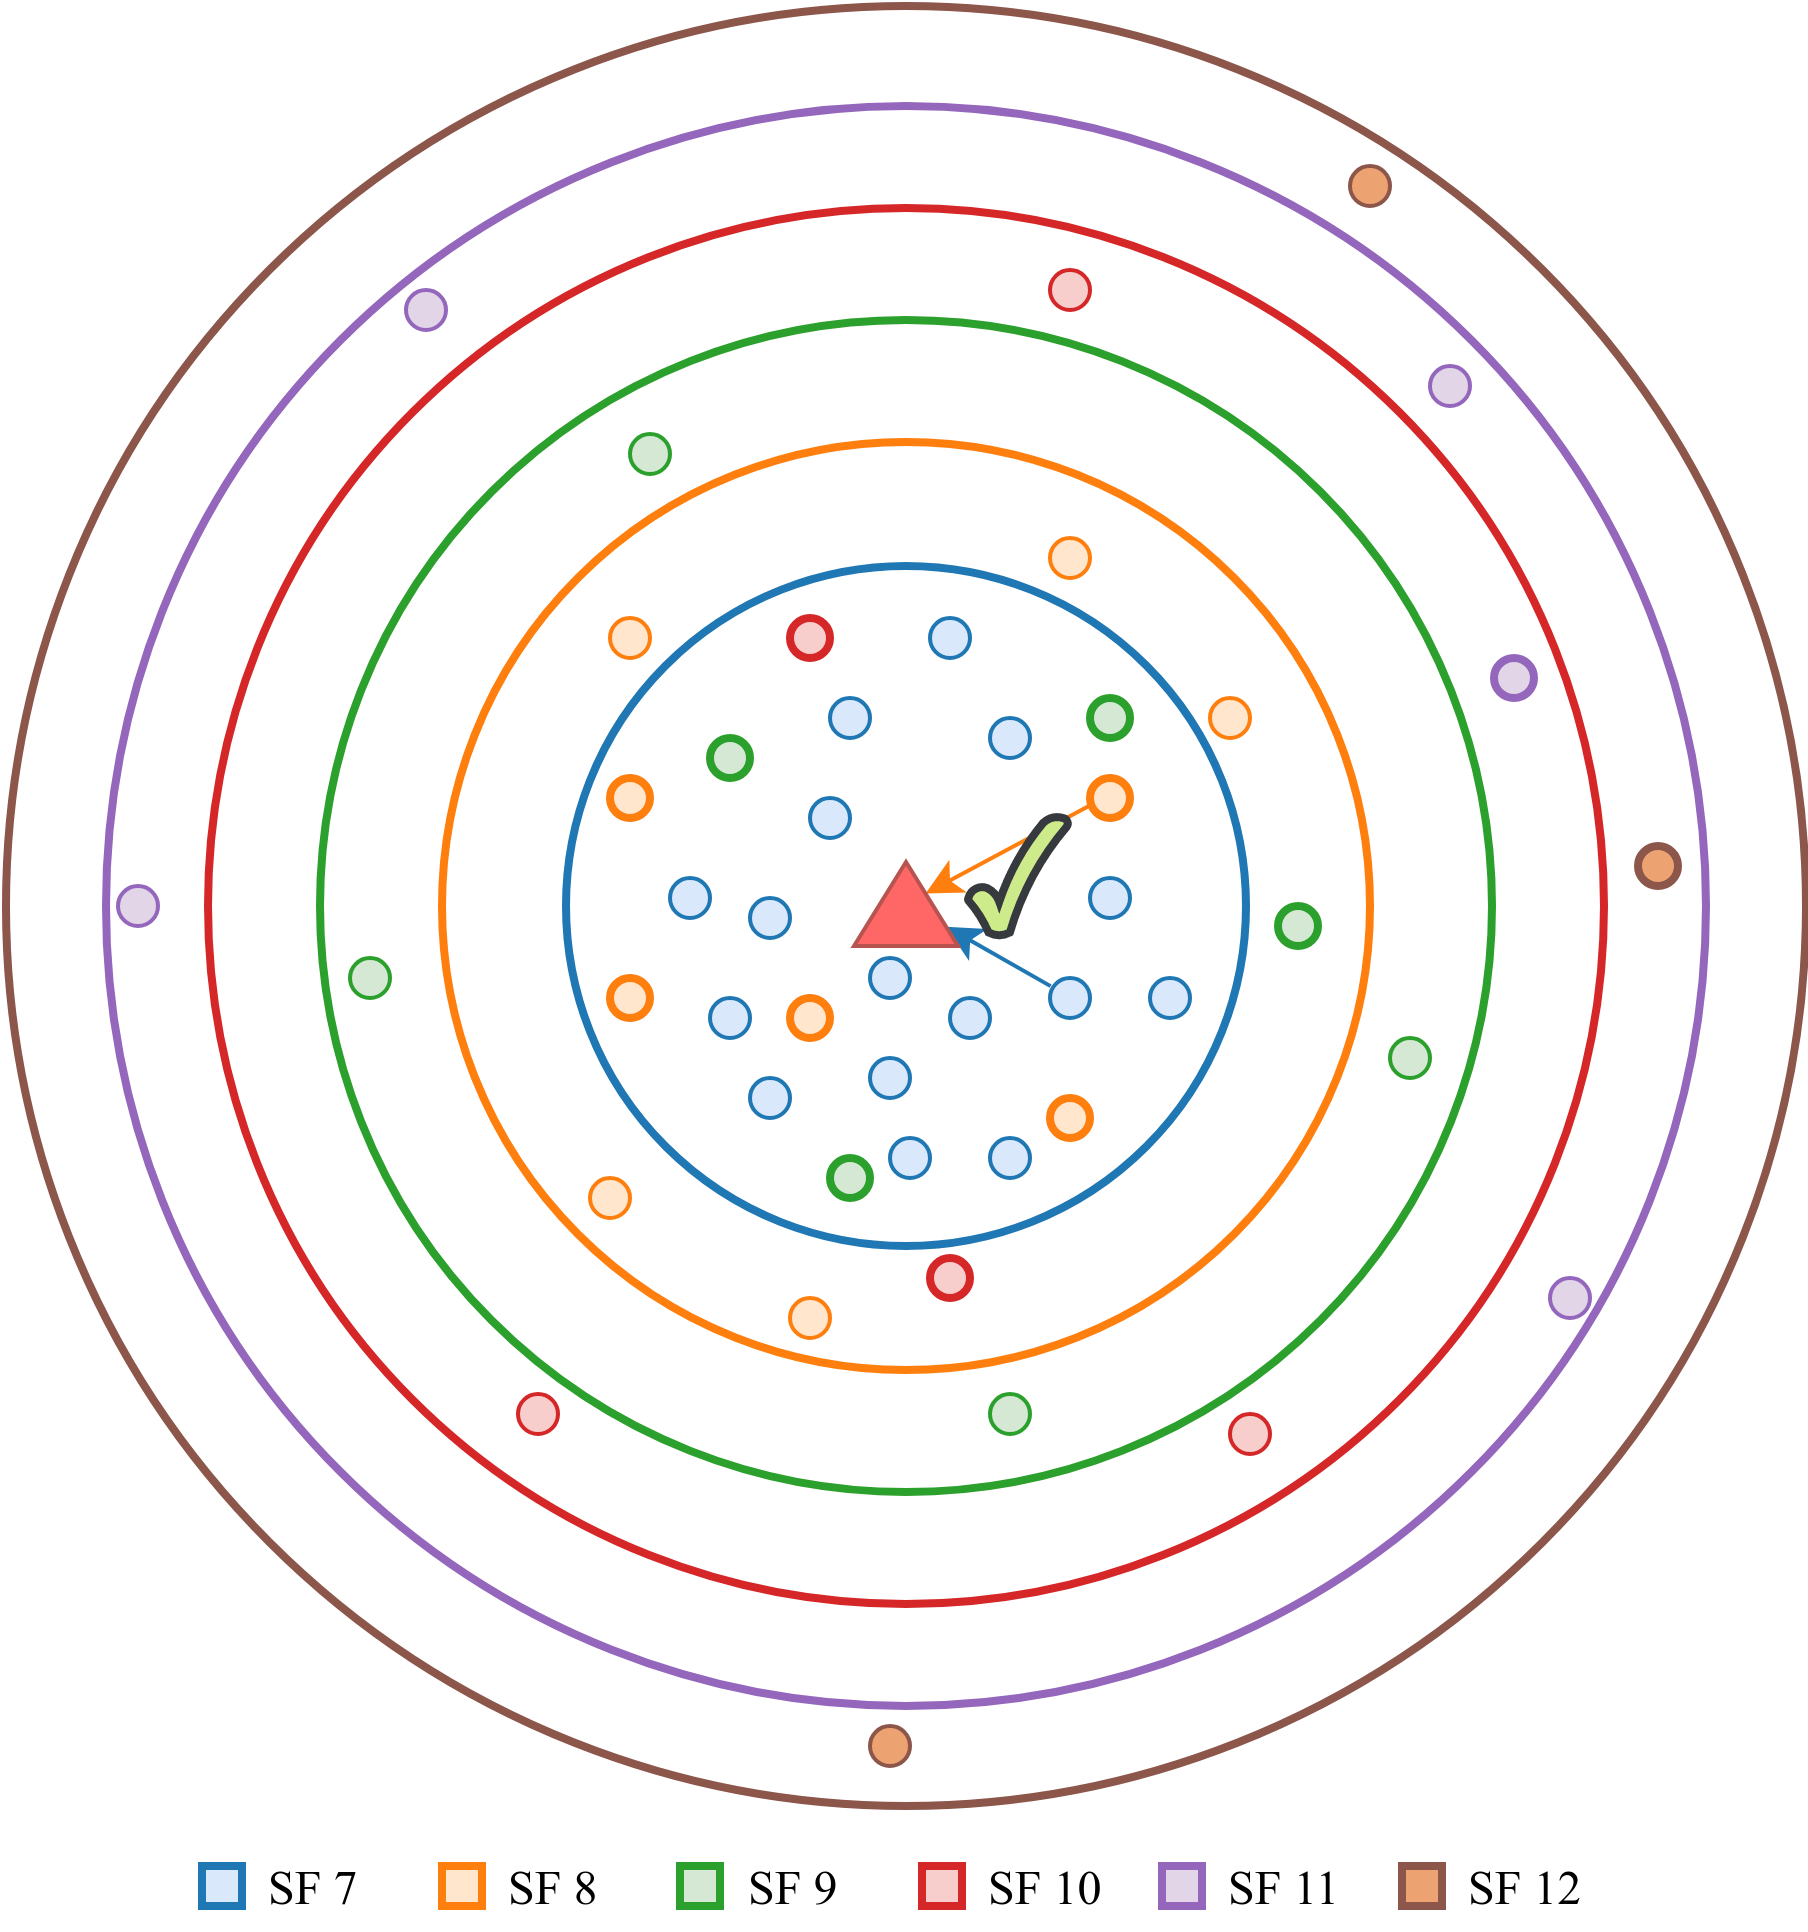
\includegraphics[width=\linewidth]{collision_solution_single_gw}
\caption{Collision avoidance proposal between nodes close to the GW by using higher SF.}
\label{fig:collision_solution_single_gw}
\end{figure}

\begin{figure}
\centering
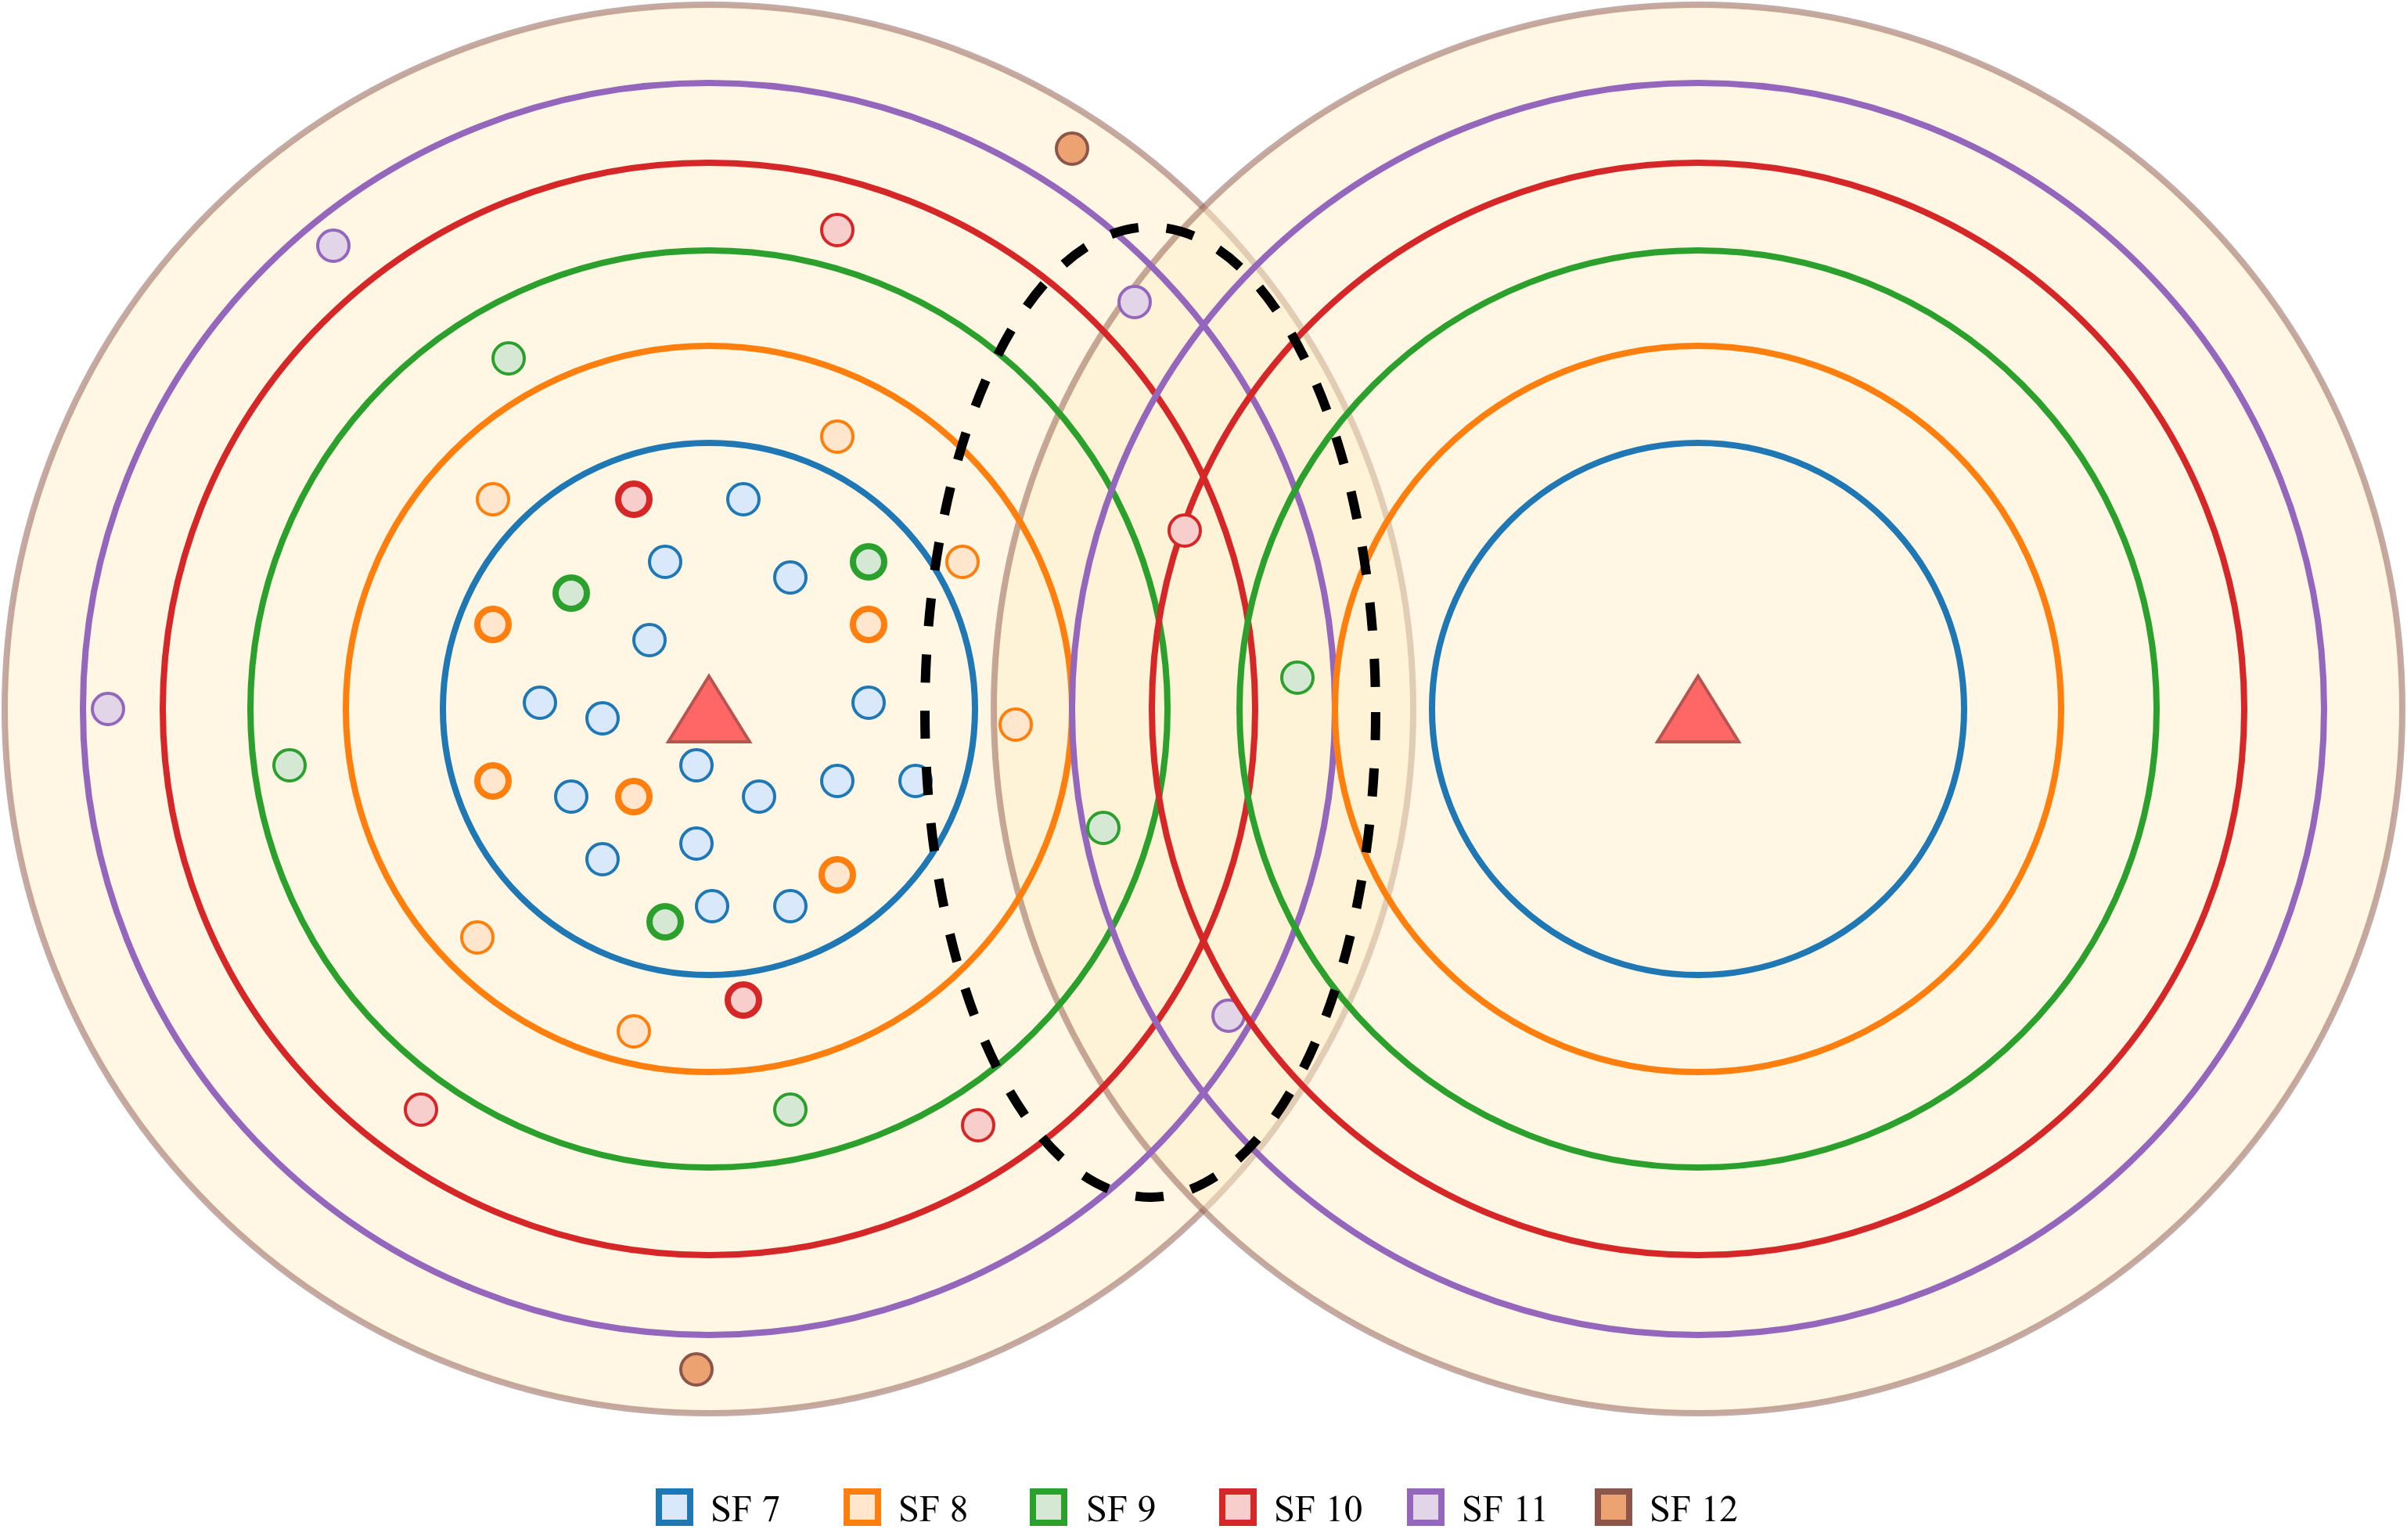
\includegraphics[width=\linewidth]{collision_solution_multi_gw}
\caption{Collision avoidance proposal for intersecting GWs.}
\label{fig:collision_solution_multi_gw}
\end{figure}


\section{Simulation Environment} \label{Simulation Environment}
\par A discrete event simulator is implemented in Python to study LoRa network performance considering SF orthogonality. The LoRaWAN SF simulation tool is publicly available at https://github.com/tugrulyatagan/simlorafs. Simulation tool supports custom LoRaWAN topologies as well as randomly generated LoRaWAN topologies. Simulator can generate uniformly distributed random circle shape network topology with radius, number of nodes and number of gateways inputs. Global simulation parameters are simulation duration (s), packet size (B), packet generation rate (p/s) and spreading factor assignment method. With these input, the simulator provide outputs of total number of generated packets, number of successfully received packet, number of interfered packets, number of under sensitivity packets, network packet delivery ratio percentage (PDR), network throughput (bps) and total transmit energy consumption (J).

\par In our simulator we only cover LoRaWAN Class A devices. Transmissions are always initiated by end nodes in pure ALOHA manner. Nodes generate a new packet according to Poisson interval for given packet rate input. In our simulator, downlink transmissions are not considered. Downlink transmissions are very rare in real world deployments since ISM band regulations dictates duty cycle transmission limit for all devices including GW. This makes downlink transmissions to very rare.

\subsection{Link Model}
\par Link quality of a wireless system can be expressed by the metric of link budget. Link budget is a measure of all gains and losses from transmitter to receiver. Link budget of a wireless link can be calculated as \cite{AN1200.22}:

\begin{equation} \label{eq:expected_rx_power}
P^{dBm}_{RX} = P^{dBm}_{TX} + G^{dB}_{SYS} - L^{dB}_{SYS} - L^{dB}_{PATH}
\end{equation}

\par Where, $P^{dBm}_{RX}$ is the expected receive power at the receiver. $P^{dBm}_{TX}$ is the transmit power of the transmitter. $G^{dB}_{SYS}$ is the system gains such as transmitter and receiver antenna gains. $L^{dB}_{SYS}$ is the system losses such as transmitter and receiver line, circuit, antenna losses. $L^{dB}_{PATH}$ is the propagation path loss between transmitter and receiver antennas in open space. In our simulation we assume that total of system gains $G^{dB}_{SYS}$ and system losses $L^{dB}_{SYS}$ is +7 dB.

\begin{table}
\centering
\caption{EU863-870 ISM Band LoRa Default Channels \cite{lorawan.regional.parameters}.}
\label{table:max_tx_power}
\begin{tabular}{|c|c|c|c|}
\hline
\textbf{Channel} & \textbf{Frequency (MHz)} & \textbf{Bandwidth (kHz)} & \textbf{Max EIRP (dBm)} \\ \hline
      1 &     868.1 &   125 &   14 \\ \hline
      2 &     868.3 &   125 &   14 \\ \hline
      3 &     868.5 &   125 &   14 \\

\hline
\end{tabular}
\end{table}

\par Maximum transmit power for European ISM band LoRa default channels can be found in Table \ref{table:max_tx_power}. In our simulator we assume that nodes are always uses maximum allowed transmit power which is 14 dBm. Different channel transmissions are independent from each other. But, in this work we focuse on SF orthogonality. Thus, we only utilized single channel transmissions in our simulator.

\begin{table}
\centering
\caption{Gateway Sensitivity for different SFs \cite{SX1276}.}
\label{table:gw_sf_sensitivity}
\begin{tabular}{|c|c|c|c|c|c|c|c|}
\hline
\multicolumn{2}{|c|}{\multirow{2}{*}{}} & \multicolumn{6}{c|}{\textbf{SF}} \\ \cline{3-8}
\multicolumn{2}{|c|}{}                  &    7 &    8 &    9 &   10 &   11 &   12 \\ \hline
\multirow{3}{*}{\textbf{BW (kHz)}}  & 125 & -123 & -126 & -129 & -132 & -133 & -136 \\ \cline{2-8}
                                    & 250 & -120 & -123 & -125 & -128 & -130 & -133 \\ \cline{2-8}
                                    & 500 & -116 & -119 & -122 & -125 & -128 & -130 \\ \hline
\end{tabular}
\end{table}

\par Receive sensitivity of a LoRa gateway for different SFs and BWs in dBm can be found in Table \ref{table:gw_sf_sensitivity} \cite{SX1276}. In our simulation, we use 125 kHz bandwidth which is also the only allowed bandwidth in EU863-870 regulation.

\par Free space propagation loss can be calculated as \cite{TR136.942}:

\begin{equation} \label{eq:propagation_loss}
\begin{split}
P^{dB}_{PATH} = 40(1 - 4 \times 10^{-3} \times h){\log_{10} R|_{km}} \\
- 18 {\log_{10} h|_{m}} + 21 {\log_{10} f|_{MHz}} + 80
\end{split}
\end{equation}

\par Where $h$ is the gateway altitude and $f$ is the frequency of the signal. We assume that $h$ = 15 m and $f$ = 868 MHz. With these assumptions, propagation loss calculation become \cite{7996384}:

\begin{equation} \label{eq:propagation_loss_simplified}
P^{dB}_{PATH} = 120.5 + 37.6 {\log_{10} R|_{km}}
\end{equation}

\par If the received signal power is higher than the gateway sensitivity, then signal can be decoded by the receiver successfully when there is no interfering transmission at the transmission period.

\subsection{Interference Model}
\par We have adopted the interference model described in \cite{7996384} to our simulator. They introduced SINR threshold matrix for modeling LoRa interference between simultaneous but different SF LoRa transmissions.

\par We assume that there is no other technology interference is present in the network except LoRa interference. To exploit imperfect orthogonality of different SF transmission, we need to calculate the effect of different SF transmissions to each other. We used signal to interference plus noise ratio (SINR) threshold matrix \cite{goursaud:hal-01231221}:

\begin{equation} \label{eq:sinr}
T = \begin{bmatrix}
       6 & -16 & -18 & -19 & -19 & -20 \\
     -24 &   6 & -20 & -22 & -22 & -22 \\
     -27 & -27 &   6 & -23 & -25 & -25 \\
     -30 & -30 & -30 &   6 & -26 & -28 \\
     -33 & -33 & -33 & -33 &   6 & -29 \\
     -36 & -36 & -36 & -36 & -36 &   6
     \end{bmatrix}
\end{equation}

\par To decide if a referenced signal is interfered at receiver by a interferer signal, we use SINR threshold matrix. $T_{i,j}$ is the needed SINR margin in dB between referenced signal with SF = i and interferer signal with SF = j to correctly decode the referenced signal. If there are more than one interferer, referenced signal must satisfy the margin for cumulative sum of all interfering signal received power values for each SF \cite{7996384}.

\begin{equation} \label{eq:sinr_db}
SINR_{i,j} = \dfrac{P_{rc,0}}{\sum_{l \in I_j} P_{rc,l}}
\end{equation}

\par Where $P_{rc,0}$ is received signal power of referenced signal and $P_{rc,l}$ is received signal power of interfering signal at SF = j. If a packet with SF = i satisfies the following condition for every SF = j, then packet is survived from all interference.

\begin{equation} \label{eq:sinr_t}
SINR_{i,j}^{dB} > T_{i,j}
\end{equation}

\par To calculate interfering power at receiver, we should consider the case where two transmissions are not perfectly overlapping. To equalize the interfering power value \cite{7996384}:

\begin{equation} \label{eq:p_interference}
P_{rc,y}^{interf} = \dfrac{P_{rc,y}(t_{interf})}{t_{x}}
\end{equation}

\par Where $t_{x}$ is transmission duration of referenced signal. $t_{interf}$ is intersection duration between referenced signal and interfering signal. Transmission duration of a packet can be calculated by data rate $R_{b}$ and packet size $PS$. Data rate of a LoRa transmission is already expressed in Equation \ref{eq:bit_rate_sf}. Duration of a LoRa transmission:

\begin{equation} \label{eq:transmission_duration}
t_{x}|_{s} = \dfrac{8 \times PS|_{B}}{R_{b}|_{bps}}
\end{equation}

\subsection{Machine Learning Model}
\par We have been able to generate mass amount of LoRaWAN transmission data for different topologies using our  tool. To come up with a solution for SF assignment issue, we have integrated a machine learning scheme to our simulator. This will allow us train a model from generated transmission data and we use this trained model to select best possible SF for nodes using prediction of the model. Tool first run a simulation with assigning random SF to nodes. Simulation results are combined into four columns which are; X and Y coordinates of the transmission source, SF of the transmission and result of the transmission. Transmission result can be successful, interfered or under sensitivity. These data is fed to Python scikit-learn decision tree classifier. After the model is created, a second simulation is run with a predictor. Model tries to find the lowest possible SF with prediction of successful transmission. 


\section{Simulation Results}  \label{Simulation Results}
\par For simulation results in this paper, we set global simulation parameters as follows. Packet size is 60 bytes including header and payload. Simulation duration is 3600 seconds.

\par In Figure \ref{fig:sf_pdr}, PDR plot of different SF assignment is shown. Randomly generated network topology radius is set to 3000 meters, number of GW is set to 1 and packet generation rate is set to 0.01 packet per second. Increasing SFs, increases time on air. This increases the number of collisions thus decreases the PDR of the network. PDR of higher SFs are decreased to almost 0 while number of node is increasing. Since network topology radius is quite small almost all SFs can reach to the GW.

\begin{figure}
\centering
\includegraphics[width=\linewidth]{{sf_pdr_r3000_g1_p0.01_s3600}.png}
\caption{PDR of different SFs.}
\label{fig:sf_pdr}
\end{figure}

\par In Figure \ref{fig:gw_pdr}, PDR plot of different number of GW is shown. Randomly generated topology radius is set to 3000 meters, packet generation rate is set to 0.01 packet per second and lowest possible SF assignment scheme is used. Increasing number of GWs, decreases the SFs of nodes and decreases time on air. This decreases number of collisions thus increases the PDR of the network when network topology radius is constant.

\begin{figure}
\centering
\includegraphics[width=\linewidth]{{gw_pdr_r3000_p0.01_s3600}.png}
\caption{PDR of different number of gateways.}
\label{fig:gw_pdr}
\end{figure}

\par In Figure \ref{fig:r_pdr}, PDR plot of different network topology radius is shown. Number of GW is set to 1, packet generation rate is set to 0.01 packet per second and lowest possible SF assignment scheme is used. Increasing network topology radius, increases the number of under sensitivity transmissions thus decreases the PDR of the network.

\begin{figure}
\centering
\includegraphics[width=\linewidth]{{r_pdr_g1_p0.01_s3600}.png}
\caption{PDR of different topology radius.}
\label{fig:r_pdr}
\end{figure}

\par In Figure \ref{fig:pr_pdr}, PDR plot of different packet generation rate is shown. Randomly generated topology radius is set to 3000 meters, number of GW is set to 1 and lowest possible SF assignment scheme is used. Increasing packet generation rate, increases the number of collisions thus decreases the PDR of the network.

\begin{figure}
\centering
\includegraphics[width=\linewidth]{{pr_pdr_r3000_g1_s3600}.png}
\caption{PDR of different packet rates.}
\label{fig:pr_pdr}
\end{figure}

\par In Figure \ref{fig:predict_pdr}, PDR plot of machine learning predictor SF scheme is shown. Randomly generated network topology radius is set to 5000 meters, number of GW is set to 3 and packet generation rate is set to 0.01 packet per second. Our predictor model needs nodes location so we simulate predictor SF scheme with at three GWs since three GWs is enough to roughly locate nodes positions by triangulation. Predictor scheme gives better PDR when number of nodes increases since number of interference increases when number of nodes increases. Predictor scheme can improve performance when LoRa interference is present. Also predictor scheme gives better results when nodes are deployed close to the gateway, since nodes have a margin to increase their SFs. If a node is far away from the GW, then predictor scheme cannot increase the SF to avoid interference since the SF is already high.

\begin{figure}
\centering
\includegraphics[width=\linewidth]{{predict_pdr_r5000_g3_p0.01_s3600}.png}
\caption{PDR of different prediction SF assignment scheme.}
\label{fig:predict_pdr}
\end{figure}


\section{Conclusion} \label{Conclusion}
\par In this paper, after brief introduction about LPWAN technologies, we provide background information about one of the most promising LPWAN technology, LoRa. Then, we discuss about LoRa modulation basics and spreading factor assignment issue. We have implemented a discrete event simulator from scratch to study network performance of LoRaWAN and evaluate different SF assignment schemes. We have shown how same SF transmission collisions can be avoided and we proposed a machine learning based solution for collision with same SF transmissions. We illustrate simulation results for proposed machine learning SF assignment technique. Our simulation results show that, proposed technique can increase network performance for dense LoRaWAN network deployed close to GWs.

\par As for future works, transmit power optimization can be included to proposed machine learning scheme. In this paper, we assume nodes always use maximum transmit power for uplink transmission, however nodes close to the GW can decrease transmit power to save energy. This will make transmission more vulnerable to interference thus requires extra care. Optimizing another node parameter alongside SF can be interesting research. Also other machine learning methods can be investigated for SF optimization. Reinforcement learning can be a good candidate for this network optimization issue.


\section*{Acknowledgment}
\par This work is supported by Turkish Ministry of Development and Istanbul Technical University researcher support program under the Grant No. ITU-AYP-2017-1.


\bibliographystyle{IEEEtran}
\bibliography{references}

\end{document}
